%%%%%%%%%%%%%%%%%%%%%%%%%%%%%%%%%%%%%%%%%%%%%%%%%%%
%% LaTeX book template                           %%
%% Author:  Amber Jain (http://amberj.devio.us/) %%
%% License: ISC license                          %%
%%%%%%%%%%%%%%%%%%%%%%%%%%%%%%%%%%%%%%%%%%%%%%%%%%%

\documentclass[a4paper,11pt,oneside]{book}
\usepackage{modulestyle}

%%%%%%%%%%%%%%%%%%%%%%%%%%%%%%%%%%%%%%%%%%%%%%%%%%%%%%%%%
% Source: http://en.wikibooks.org/wiki/LaTeX/Hyperlinks %
%%%%%%%%%%%%%%%%%%%%%%%%%%%%%%%%%%%%%%%%%%%%%%%%%%%%%%%%%

%%%%%%%%%%%%%%%%%%%%%%%%%%%%%%%%%%%%%%%%%%%%%%%%%%%%%%%%%%%%%%%%%%%%%%%%%%%%%%%%
% 'dedication' environment: To add a dedication paragraph at the start of book %
% Source: http://www.tug.org/pipermail/texhax/2010-June/015184.html            %
%%%%%%%%%%%%%%%%%%%%%%%%%%%%%%%%%%%%%%%%%%%%%%%%%%%%%%%%%%%%%%%%%%%%%%%%%%%%%%%%
\newenvironment{dedication}
{
   \cleardoublepage
   \thispagestyle{empty}
   \vspace*{\stretch{1}}
   \hfill\begin{minipage}[t]{0.66\textwidth}
   \raggedright
}
{
   \end{minipage}
   \vspace*{\stretch{3}}
   \clearpage
}

%%%%%%%%%%%%%%%%%%%%%%%%%%%%%%%%%%%%%%%%%%%%%%%%
% Chapter quote at the start of chapter        %
% Source: http://tex.stackexchange.com/a/53380 %
%%%%%%%%%%%%%%%%%%%%%%%%%%%%%%%%%%%%%%%%%%%%%%%%
\makeatletter
\renewcommand{\@chapapp}{}% Not necessary...
\newenvironment{chapquote}[2][2em]
  {\setlength{\@tempdima}{#1}%
   \def\chapquote@author{#2}%
   \parshape 1 \@tempdima \dimexpr\textwidth-2\@tempdima\relax%
   \itshape}
  {\par\normalfont\hfill--\ \chapquote@author\hspace*{\@tempdima}\par\bigskip}
\makeatother

%%%%%%%%%%%%%%%%%%%%%%%%%%%%%%%%%%%%%%%%%%%%%%%%%%%
% First page of book which contains 'stuff' like: %
%  - Book title, subtitle                         %
%  - Book author name                             %
%%%%%%%%%%%%%%%%%%%%%%%%%%%%%%%%%%%%%%%%%%%%%%%%%%%

\newcommand{\BookTitle}{Applications Development and Emerging Technologies}
\newcommand{\BookTitleFootnote}{A course in the Bachelor of Science in Computer Science.}

\newcommand{\BookSubtitle}{A Study Guide for Students of Sorsogon State University - Bulan Campus}
\newcommand{\BookSubtitleFootnote}{This book is a study guide for students of
Sorsogon State University - Bulan Campus taking up the course Applications Development and Emerging Technologies.}

\newcommand{\BookAuthorFirstName}{Jarrian Vince}
\newcommand{\BookAuthorLastName}{Gojar}
\newcommand{\BookAuthorName}{Jarrian Vince G. Gojar}
\newcommand{\BookAuthorURL}{https://github.com/godkingjay}

% Book's title and subtitle
\title{\Huge \textbf{\BookTitle}  \footnote{\BookTitleFootnote} \\
\huge \BookSubtitle \footnote{\BookSubtitleFootnote}}

% Author
\author{\textsc{\BookAuthorName}\thanks{\url{\BookAuthorURL}}}

\begin{document}

\frontmatter
\maketitle

%%%%%%%%%%%%%%%%%%%%%%%%%%%%%%%%%%%%%%%%%%%%%%%%%%%%%%%%%%%%%%%
% Add a dedication paragraph to dedicate your book to someone %
%%%%%%%%%%%%%%%%%%%%%%%%%%%%%%%%%%%%%%%%%%%%%%%%%%%%%%%%%%%%%%%
\begin{dedication}
Sorsogon State University - Bulan Campus
\end{dedication}

%%%%%%%%%%%%%%%%%%%%%%%%%%%%%%%%%%%%%%%%%%%%%%%%%%%%%%%%%%%%%%%%%%%%%%%%
% Auto-generated table of contents, list of figures and list of tables %
%%%%%%%%%%%%%%%%%%%%%%%%%%%%%%%%%%%%%%%%%%%%%%%%%%%%%%%%%%%%%%%%%%%%%%%%
\tableofcontents
\listoffigures
\listoftables
\lstlistoflistings

\mainmatter

%%%%%%%%%%%
% Preface %
%%%%%%%%%%%
\chapter*{Preface}
% A Quote all about Applications Development and Emerging Technologies
\begin{chapquote}{}
\end{chapquote}

\noindent \BookAuthorName \\
\noindent \url{\BookAuthorURL}

%%%%%%%%%%%%%%%%%%%%%%%%%%%%%%%%%%%%
%%%%%~ NEW CHAPTER STARTS HERE %%%%%
%%%%%%%%%%%%%%%%%%%%%%%%%%%%%%%%%%%%
\chapter{Introduction to Applications Development and Emerging Technologies}

\section{Introduction}

\subsection{Application}

An \textbf{application} is a software program that allows users to
perform specific tasks. Applications for desktop or laptop computers
are sometimes called \textbf{desktop applications}, while those for
mobile devices are called \textbf{mobile apps}. When you open an 
application, it runs inside the operating system until you close it.
Most of the time, you will have more than one application open at
the same time, which is known as \textbf{multitasking}.

\subsection{Development}

\textbf{Development} is the process of creating a software application.
It includes designing the user interface, writing code, and testing
the application for bugs. The goal of software development is to
create a program that is easy to use and works correctly.

\subsection{Application Development}

\textbf{Application development} is the process of planning, designing,
creating, testing, and deploying an application to perform various
business operations. It can be done by massive organizations with large
teams working on projects or by a single freelance developer.

% \section{Software Development Life Cycle}

% The \textbf{software development life cycle} (SDLC) is a process used by
% software developers to design, develop, and test software applications.
% The SDLC consists of several phases, including planning, analysis, design,
% implementation, and maintenance.

% \subsection{Different Types of Software Development Life Cycle Models}

% There are several different types of software development life cycle models,
% including:

% \begin{itemize}
%   \item Waterfall Model
%   \item Agile Model
%   \item Spiral Model
%   \item V-Model
%   \item Iterative Model
% \end{itemize}

% \subsubsection{Waterfall Model}

% The \textbf{waterfall model} is a linear and sequential approach to software
% development. It consists of several phases, including requirements gathering,
% analysis, design, coding/implementation, testing, and maintenance. Each phase
% must be completed before moving on to the next phase.

% % Image from ./assets/sdlc/waterfall.png
% \begin{figure}[H]
%   \centering
%   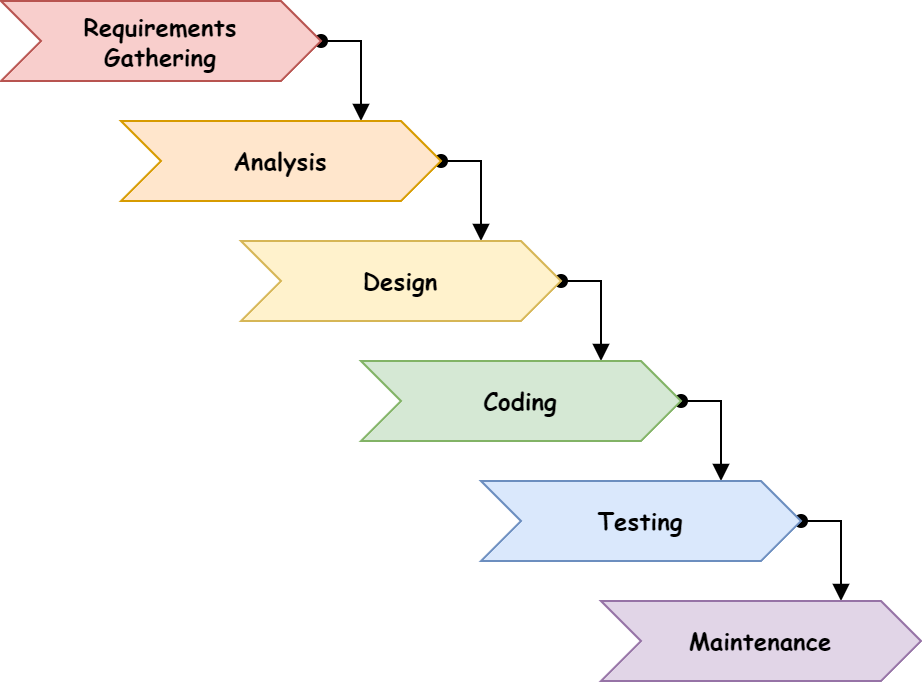
\includegraphics[width=1\textwidth]{./assets/sdlc/waterfall.png}
%   \caption{Waterfall Model}
%   \label{fig:waterfall}
% \end{figure}

% Figure \ref{fig:waterfall} shows the waterfall model.

% \begin{itemize}
%   \item \textbf{Requirements Gathering:} In this phase, the requirements
%   for the software application are gathered from the client or end-users.
%   This phase answers the question, "What does the customer want?".

%   \item \textbf{Analysis:} In this phase, the requirements gathered in the
%   previous phase are analyzed to determine the feasibility of the project.
%   This phase answers the question, "What is the best way to achieve the
%   customer's requirements?".

%   \item \textbf{Design:} In this phase, the software application is
%   designed based on the requirements gathered in the previous phases.
%   This phase answers the question, "How will the software application
%   look and function?".

%   \item \textbf{Coding/Implementation:} In this phase, the software
%   application is developed based on the design created in the previous
%   phase. This phase answers the question, "How will the software
%   application be built?".

%   \item \textbf{Testing:} In this phase, the software application is
%   tested to ensure that it works correctly and meets the requirements
%   specified by the client or end-users. This phase answers the question,
%   "Does the software application work as expected?".

%   \item \textbf{Maintenance:} In this phase, the software application is
%   maintained and updated to fix any bugs or issues that arise after the
%   application has been deployed. This phase answers the question, "How
%   can the software application be improved?".
% \end{itemize}

% \subsubsection{Agile Model}

% The \textbf{agile model} is an iterative and incremental approach to
% software development. It consists of several phases, including planning,
% design, coding, testing, and deployment. The agile model allows for
% flexibility and adaptability throughout the development process.

% % Image from ./assets/sdlc/agile.png

\section{Different Types of Application Development}

There are several different types of application development, including:

\begin{itemize}
  \item Web Development
  \item Mobile Application Development
  \item Desktop Application Development
  \item Game Development
  \item Cloud Development
\end{itemize}

\subsection{Web Development}

\textbf{Web development} is the process of creating websites and web
applications. It involves designing the user interface, writing code,
and testing the website for bugs. Web development can be divided into
two categories: front-end development and back-end development.

\subsubsection{Front-End Development}

\textbf{Front-end development} is the process of creating the user
interface of a website. It involves designing the layout, colors, and
fonts of the website. Front-end developers use HTML, CSS, and JavaScript
to create the user interface of a website.

\begin{enumerate}
  \item \textbf{HTML (HyperText Markup Language)} is the standard markup
  language used to create web pages. It defines the structure of a web
  page using a series of elements.

  \item \textbf{CSS (Cascading Style Sheets)} is a style sheet language
  used to define the appearance of a web page. It allows developers to
  control the layout, colors, and fonts of a website.

  \item \textbf{JavaScript} is a programming language used to create
  interactive elements on a web page. It allows developers to add
  functionality such as animations, pop-ups, and form validation to a
  website.

  \item \textbf{Bootstrap} is a front-end framework that allows developers
  to create responsive and mobile-first websites. It provides a set of
  pre-designed components, such as buttons, forms, and navigation bars,
  that can be easily customized.

  \item \textbf{React} is a JavaScript library used to create user
  interfaces for single-page applications. It allows developers to build
  reusable components that update automatically when the data changes.

  \item \textbf{Angular} is a front-end framework that allows developers
  to create dynamic web applications. It provides a set of tools and
  libraries for building interactive user interfaces.

  \item \textbf{Vue} is a progressive JavaScript framework used to create
  user interfaces and single-page applications. It allows developers to
  build interactive web applications with ease.
\end{enumerate}

The above tools and technologies are commonly used in front-end development
to create responsive and interactive websites. HTML, CSS, and JavaScript
are the building blocks of front-end development, while frameworks such
as Bootstrap, React, Angular, and Vue provide additional features for
building modern web applications.

\subsubsection{Back-End Development}

\textbf{Back-end development} is the process of creating the server-side
logic of a website. It involves writing code that interacts with the
database and processes data. Back-end developers use programming languages
such as PHP, Python, and Ruby to create the server-side logic of a website.

\begin{enumerate}
  \item \textbf{Node.js} is a JavaScript runtime environment that allows
  developers to run JavaScript on the server-side. It provides a set of
  libraries and tools for building scalable and high-performance web
  applications.

  \item \textbf{Express} is a web application framework for Node.js. It
  provides a set of features for building web applications, such as routing,
  middleware, and templating.

  \item \textbf{Django} is a high-level web framework for Python. It allows
  developers to build web applications quickly and efficiently. Django
  provides a set of tools and libraries for building secure and scalable
  web applications.

  \item \textbf{Flask} is a lightweight web framework for Python. It allows
  developers to build web applications with minimal code. Flask provides
  a set of tools and libraries for building simple and scalable web
  applications.

  \item \textbf{Ruby on Rails} is a web application framework for Ruby. It
  provides a set of tools and libraries for building web applications
  quickly and efficiently. Ruby on Rails follows the convention over
  configuration principle, which allows developers to write less code
  and focus on building the application.

  \item \textbf{Laravel} is a web application framework for PHP. It
  provides a set of tools and libraries for building web applications
  quickly and efficiently. Laravel follows the model-view-controller
  (MVC) architecture, which allows developers to separate the business
  logic from the presentation layer.

  \item \textbf{Spring} is a web application framework for Java. It
  provides a set of tools and libraries for building enterprise-level
  web applications. Spring follows the inversion of control (IoC)
  principle, which allows developers to write loosely coupled code
  and focus on building the application.
\end{enumerate}

The above tools and technologies are commonly used in back-end development
to create the server-side logic of a website. Back-end developers use
these tools to interact with the database, process data, and handle
user requests on the server-side.

\subsection{Mobile Application Development}

\textbf{Mobile application development} is the process of creating mobile applications
for smartphones and tablets. It involves designing the user interface,
writing code, and testing the mobile application for bugs. Mobile
development can be divided into two categories: iOS development and
Android development.

\subsubsection{iOS Development}

\textbf{iOS development} is the process of creating mobile applications
for Apple devices, such as iPhones and iPads. It involves designing the
user interface using Xcode and writing code in Swift or Objective-C.
iOS developers use Xcode, Swift, and Objective-C to create mobile
applications for Apple devices.

\begin{enumerate}
  \item \textbf{Xcode} is an integrated development environment (IDE)
  used to create iOS applications. It provides a set of tools and
  libraries for building mobile applications for Apple devices.

  \item \textbf{Swift} is a programming language used to create iOS
  applications. It provides a set of features for building mobile
  applications, such as type safety, optionals, and generics.

  \item \textbf{Objective-C} is a programming language used to create
  iOS applications. It provides a set of features for building mobile
  applications, such as dynamic typing, message passing, and memory
  management.

  \item \textbf{React Native} is a JavaScript framework used to create
  mobile applications for Android and iOS devices. It allows developers
  to build cross-platform mobile applications with a single codebase.

  \item \textbf{Flutter} is a mobile UI framework used to create mobile
  applications for Android and iOS devices. It allows developers to build
  cross-platform mobile applications with a single codebase.
\end{enumerate}

The above tools and technologies are commonly used in iOS development
to create mobile applications for Apple devices. iOS developers use
these tools to design the user interface and write code for mobile
applications.

\subsubsection{Android Development}

\textbf{Android development} is the process of creating mobile
applications for Android devices. It involves designing the user
interface using Android Studio and writing code in Java or Kotlin.
Android developers use Android Studio, Java, and Kotlin to create
mobile applications for Android devices.

\begin{enumerate}
  \item \textbf{Android Studio} is an integrated development environment
  (IDE) used to create Android applications. It provides a set of tools
  and libraries for building mobile applications for Android devices.

  \item \textbf{Java} is a programming language used to create Android
  applications. It provides a set of features for building mobile
  applications, such as object-oriented programming, inheritance, and
  polymorphism.

  \item \textbf{Kotlin} is a programming language used to create Android
  applications. It provides a set of features for building mobile
  applications, such as null safety, extension functions, and coroutines.

  \item \textbf{React Native} is a JavaScript framework used to create
  mobile applications for Android and iOS devices. It allows developers
  to build cross-platform mobile applications with a single codebase.

  \item \textbf{Flutter} is a mobile UI framework used to create mobile
  applications for Android and iOS devices. It allows developers to build
  cross-platform mobile applications with a single codebase.
\end{enumerate}

The above tools and technologies are commonly used in Android development
to create mobile applications for Android devices. Some of the tools here
are also used in iOS development to create mobile applications for Apple
devices. React Native and Flutter in particular are used to build
cross-platform mobile applications for both Android and iOS devices.

\subsection{Desktop Application Development}

\textbf{Desktop application development} is the process of creating desktop
applications for Windows, macOS, and Linux. It involves designing the
user interface, writing code, and testing the desktop application for
bugs.

\begin{enumerate}
  \item \textbf{Electron} is a framework used to create desktop
  applications with web technologies. It allows developers to build
  cross-platform desktop applications with HTML, CSS, and JavaScript.

  \item \textbf{JavaFX} is a framework used to create desktop applications
  with Java. It provides a set of tools and libraries for building
  cross-platform desktop applications with Java.

  \item \textbf{Qt} is a framework used to create desktop applications
  with C++. It provides a set of tools and libraries for building
  cross-platform desktop applications with C++.

  \item \textbf{WinForms} is a framework used to create desktop
  applications with C\#. It provides a set of tools and libraries for
  building desktop applications for Windows.

  \item \textbf{WPF} is a framework used to create desktop applications
  with C\#. It provides a set of tools and libraries for building
  desktop applications for Windows.
\end{enumerate}

The above tools and technologies are commonly used in desktop development
to create desktop applications for Windows, macOS, and Linux. For
Windows, developers use WinForms and WPF to create desktop applications
with C\#. For cross-platform desktop applications, developers use
Electron, JavaFX, and Qt to build desktop applications with web
technologies, Java, and C++.

\subsection{Game Development}

\textbf{Game development} is the process of creating video games for
consoles, computers, and mobile devices. It involves designing the
gameplay, writing code, and testing the game for bugs.

\begin{enumerate}
  \item \textbf{Unity} is a game engine used to create 2D and 3D games
  for consoles, computers, and mobile devices. It provides a set of
  tools and libraries for building cross-platform games with C\#.

  \item \textbf{Unreal Engine} is a game engine used to create 2D and
  3D games for consoles, computers, and mobile devices. It provides a
  set of tools and libraries for building cross-platform games with C++.

  \item \textbf{Godot} is a game engine used to create 2D and 3D games
  for consoles, computers, and mobile devices. It provides a set of
  tools and libraries for building cross-platform games with GDScript.

  \item \textbf{GameMaker Studio} is a game engine used to create 2D
  games for consoles, computers, and mobile devices. It provides a set
  of tools and libraries for building cross-platform games with GML.

  \item \textbf{Construct} is a game engine used to create 2D games for
  consoles, computers, and mobile devices. It provides a set of tools
  and libraries for building cross-platform games with events.
\end{enumerate}

The above tools and technologies are commonly used in game development
to create video games for consoles, computers, and mobile devices. Unity,
Unreal Engine, Godot, GameMaker Studio, and Construct are popular game
engines used by game developers to create 2D and 3D games. These game
engines provide a set of tools and libraries for building cross-platform
games with C\#, C++, GDScript, and GML.

\subsection{Cloud Development}

\textbf{Cloud development} is the process of creating cloud-based
applications that run on remote servers. It involves designing the
user interface, writing code, and testing the cloud application for
bugs.

\begin{enumerate}
  \item \textbf{Amazon Web Services (AWS)} is a cloud platform used to
  create cloud-based applications. It was one of the first cloud
  platforms and is widely used by developers to build scalable and
  secure cloud applications. It is a subsidiary of Amazon providing
  on-demand cloud computing platforms and APIs to individuals,

  \item \textbf{Microsoft Azure}, similarly to AWS, is a cloud platform
  used to create cloud-based applications. Microsoft Azure is a cloud
  computing service created by Microsoft for building, testing, deploying,
  and managing applications and services through Microsoft-managed data
  centers.

  \item \textbf{Google Cloud Platform (GCP)}, similarly to AWS and
  Microsoft Azure, is a cloud platform used to create cloud-based
  applications. Google Cloud Platform is a suite of cloud computing
  services that runs on the same infrastructure that Google uses
  internally for its end-user products, such as Google Search, Gmail,
  file storage, and YouTube.

  \item \textbf{Heroku} is a cloud platform used to create cloud-based
  applications. It provides a set of tools and services for building
  scalable and secure cloud applications. Heroku is a cloud platform
  as a service supporting several programming languages.

  \item \textbf{Firebase}, also developed by Google, is a cloud
  platform used to create cloud-based applications. Firebase is a
  platform developed by Google for creating mobile and web applications.
  It was originally an independent company founded in 2011. In 2014,
  Google acquired the platform and it is now their flagship offering
  for app development.
\end{enumerate}

The above tools and technologies are commonly used in cloud development
to create cloud-based applications that run on remote servers. AWS,
Microsoft Azure, GCP, Heroku, and Firebase are popular cloud platforms
used by developers to build scalable and secure cloud applications. These
cloud platforms provide a set of tools and services for building
cloud-based applications with ease.

\chapter{Web Development}

\section{Introduction}

There are around 3.58 billion internet users on the planet. This implies
that over half of the world's 7.6 billion people have access to the
internet, which they use for everything from entertainment to education,
communication to commerce, keeping up with current events, and keeping
up with business experts. Indeed, for most people, the internet is the 
first (and often only) channel through which we communicate with the
world in all of its complexities.

There are three interactive elements on the internet:

\begin{enumerate}
  \item \textbf{Websites} - A collection of web pages that are linked
  together and share a common domain name.

  \item \textbf{Servers} - A computer or computer program that manages
  access to a centralized resource or service in a network.

  \item \textbf{Browsers} - A software application used to access and
  view websites on the internet.
\end{enumerate}

The frontend (client side) and the backend (server side) are two parts of any
website. The frontend comprises everything the user sees and experiences
instantly while visiting a website. The backend is behind the scenes that store,
send and receive information.

HTML, CSS, and Javascript files make up everything a user sees on a website.
As a web developer, these are the most basic tools needed. They are the
languages that required to build websites.

\section{HTML}

\textbf{HTML (HyperText Markup Language)} is the standard markup language
used to create web pages. It defines the structure of a web page using a
series of elements. It contains the essential elements of a website, such
as words, titles, and paragraphs, as well as links, images, and other
media. HTML elements are represented by tags, which are enclosed in angle
brackets. HTML forms the backbone of any webpage, dictating its structure
and content.

\begin{lstlisting}[language=HTML, caption={HTML Example}, label={lst:html-example}]
<!DOCTYPE html>
<html lang="en">

<head>
    <meta charset="UTF-8" />
    <meta name="viewport" content="width=device-width, initial-scale=1.0" />
    <title>First Web Page</title>
</head>

<body>
    <h1>Hello, World!</h1>
    <p>Welcome to my website.</p>
</body>

</html>
\end{lstlisting}

Code \ref{lst:html-example} shows an example of an HTML document. An
HTML boilerplate usually looks like this:

\begin{itemize}
  \item \textbf{<!DOCTYPE html>} - Defines the document type and version
  of HTML. In this case, it is HTML5.
  \item \textbf{<html>} - Defines the root element of an HTML page.
  \item \textbf{<head>} - Contains meta-information about the document,
  such as the title, character set, and viewport.
  \item \textbf{<body>} - Contains the content of the document, such as
  headings, paragraphs, and images.
\end{itemize}

\subsection{HTML Tags}

HTML tags are used to define the structure and content of a web page.
They are enclosed in angle brackets and come in pairs: an opening tag
and a closing tag. The opening tag is used to define the beginning of
an element, while the closing tag is used to define the end of an element.

\subsubsection{<html>...</html>}

This tag specifies that the webpage is written
in HTML. It appears at the very first and last line
of the webpage. It is mainly used to show that
the page uses HTML5 – the latest version of
the language. Also known as the root element,
this tag can be thought of as a parent tag for
every other tag used in the page.

\begin{lstlisting}[language=HTML, caption={HTML <html> Tag}, label={lst:html-tag}]
<!DOCTYPE html>
<html lang="en">
    <!-- Content goes here -->
</html>
\end{lstlisting}

Code \ref{lst:html-tag} shows an example of the <html> tag. Here, the
\textbf{lang} attribute specifies the language of the document, which
is English in this case.

\subsubsection{<head>...</head>}

This tag is used to define the head section of the
webpage. The head section contains meta-information
about the document, such as the title, character set,
and viewport. It is not displayed on the webpage but
is used to provide information about the document to
the browser and search engines.

\begin{lstlisting}[language=HTML, caption={HTML <head> Tag}, label={lst:head-tag}]
<head>
    <meta charset="UTF-8" />
    <meta name="viewport" content="width=device-width, initial-scale=1.0" />
    <title>First Web Page</title>
</head>
\end{lstlisting}

Code \ref{lst:head-tag} shows an example of the <head> tag. Here, the
\textbf{<meta>} tag is used to define the character set and viewport of
the document, while the \textbf{<title>} tag is used to define the title
of the document. This title appears in the browser tab.

\subsubsection{<title>...</title>}

This tag is used to define the title of the document.
It appears in the browser tab and is used to identify
the webpage.

\begin{lstlisting}[language=HTML, caption={HTML <title> Tag}, label={lst:title-tag}]
<title>First Web Page</title>
\end{lstlisting}

Code \ref{lst:title-tag} shows an example of the <title> tag. Here, the
title of the document is "First Web Page". This title appears in the
browser tab when the document is opened.

\subsubsection{<body>...</body>}

This tag is used to define the body section of the
webpage. The body section contains the content of
the document, such as headings, paragraphs, and
images. It is displayed on the webpage and is
visible to the user.

\begin{lstlisting}[language=HTML, caption={HTML <body> Tag}, label={lst:body-tag}]
<body>
    <h1>Hello, World!</h1>
    <p>Welcome to my website.</p>
</body>
\end{lstlisting}

Code \ref{lst:body-tag} shows an example of the <body> tag. Here, the
\textbf{<h1>} tag is used to define a heading, while the \textbf{<p>}
tag is used to define a paragraph. This content is displayed on the
webpage and is visible to the user.

\subsubsection{<h1>...</h1> to <h6>...</h6>}

These tags are used to define headings of different
sizes. The \textbf{<h1>} tag defines the largest heading,
while the \textbf{<h6>} tag defines the smallest heading.
Headings are used to define the structure of the document
and provide a hierarchy of information.

\begin{lstlisting}[language=HTML, caption={HTML <h1> to <h6> Tags}, label={lst:h-tag}]
<h1>This is a Heading 1</h1>
<h2>This is a Heading 2</h2>
<h3>This is a Heading 3</h3>
<h4>This is a Heading 4</h4>
<h5>This is a Heading 5</h5>
<h6>This is a Heading 6</h6>
\end{lstlisting}

Code \ref{lst:h-tag} shows an example of the \textbf{<h1>} to
\textbf{<h6>} tags. These tags are used to define headings of
different sizes, with \textbf{<h1>} being the largest and
\textbf{<h6>} being the smallest.

\subsubsection{<p>...</p>}

This tag is used to define a paragraph of text. It is
used to group text content together and provide structure
to the document.

\begin{lstlisting}[language=HTML, caption={HTML <p> Tag}, label={lst:p-tag}]
<p>
  Excepteur officia tempor do laborum commodo cupidatat ea Lorem qui irure enim velit. Adipisicing dolor minim Lorem nulla dolor quis et aliqua. Officia anim adipisicing excepteur sint elit qui laboris reprehenderit non elit. Voluptate voluptate duis aliqua proident elit exercitation cillum anim reprehenderit nostrud minim culpa veniam.
</p>
\end{lstlisting}

Code \ref{lst:p-tag} shows an example of the \textbf{<p>} tag. This tag
is used to define a paragraph of text, which is displayed on the webpage.

\subsubsection{<div>...</div>}

This tag is used to define a division or section of
the document. It is a block-level element that can
contain other block-level or inline elements.

\begin{lstlisting}[language=HTML, caption={HTML <div> Tag}, label={lst:div-tag}]
<div>
    <h1>Hello, World!</h1>
    <p>Welcome to my website.</p>
</div>

<div>
    <img src="https://avatar.iran.liara.run/public/boy" alt="Image" />
    <img src="https://avatar.iran.liara.run/public/girl" alt="Image" />
</div>
\end{lstlisting}

Code \ref{lst:div-tag} shows an example of the \textbf{<div>} tag. This
tag is used to define a division or section of the document, which can
contain other elements such as headings, paragraphs, and images.

\subsubsection{<section>...</section>}

This tag is used to define a section of the document.
It is usually used to group related content together
such as articles, blog posts, or product listings.

\begin{lstlisting}[language=HTML, caption={HTML <section> Tag}, label={lst:section-tag}]
<section>
    <h2>Section 1</h2>
    <p>Content for section 1 goes here.</p>
</section>

<section>
    <h2>Section 2</h2>
    <p>Content for section 2 goes here.</p>
</section>

<section>
    <h2>Section 3</h2>
    <p>Content for section 3 goes here.</p>
</section>
\end{lstlisting}

Code \ref{lst:section-tag} shows an example of the \textbf{<section>} tag.
This tag is used to define a section of the document, which can contain
related content such as headings and paragraphs.

\subsubsection{<span>...</span>}

This tag is used to define a span of text. It is an
inline element that can contain other inline elements.

\begin{lstlisting}[language=HTML, caption={HTML <span> Tag}, label={lst:span-tag}]
<p>Welcome to my <span>website</span>.</p>
\end{lstlisting}

Code \ref{lst:span-tag} shows an example of the \textbf{<span>} tag. This
tag is used to define a span of text, which can be styled separately from
the rest of the paragraph.

\subsubsection{<br />}
This tag is used to insert a line break in the document.
It is a self-closing tag that does not require a closing tag.

\begin{lstlisting}[language=HTML, caption={HTML <br /> Tag}, label={lst:br-tag}]
<p>Welcome to my <br /> website.</p>
\end{lstlisting}

Code \ref{lst:br-tag} shows an example of the \textbf{<br />} tag. This
tag is used to insert a line break in the document, which moves the
content to the next line.

\subsubsection{<hr />}

This tag is used to insert a horizontal rule in the
document. It is a self-closing tag that creates a
horizontal line across the page.

\begin{lstlisting}[language=HTML, caption={HTML <hr /> Tag}, label={lst:hr-tag}]
<p>Welcome to my website.</p>
<hr />
<p>Thank you for visiting.</p>
\end{lstlisting}

Code \ref{lst:hr-tag} shows an example of the \textbf{<hr />} tag. This
tag is used to insert a horizontal rule in the document, which creates
a horizontal line across the page.

\subsubsection{<img />}

This tag is used to insert an image in the document.
It is a self-closing tag that requires the \textbf{src}
attribute to specify the image file.

\begin{lstlisting}[language=HTML, caption={HTML <img /> Tag}, label={lst:img-tag}]
<img src="https://avatar.iran.liara.run/public" alt="Image" />
\end{lstlisting}

Code \ref{lst:img-tag} shows an example of the \textbf{<img />} tag. This
tag is used to insert an image in the document, which is displayed on the
webpage. The \textbf{src} attribute specifies the image file, while the
\textbf{alt} attribute provides alternative text for the image.

\subsubsection{<a>...</a>}

This tag is used to create a hyperlink in the document.
It requires the \textbf{href} attribute to specify the
URL of the link.

\begin{lstlisting}[language=HTML, caption={HTML <a> Tag}, label={lst:a-tag}]
<a href="https://www.github.com/godkingjay">Visit GitHub</a>
\end{lstlisting}

Code \ref{lst:a-tag} shows an example of the \textbf{<a>} tag. This tag
is used to create a hyperlink in the document, which links to the
specified URL. The \textbf{href} attribute specifies the URL of the link.

\subsubsection{<ul>...</ul>}

This tag is used to create an unordered list in the
document. It contains a list of items that are displayed
with bullet points.

\begin{lstlisting}[language=HTML, caption={HTML <ul> Tag}, label={lst:ul-tag}]
<ul>
    <li>Item 1</li>
    <li>Item 2</li>
    <li>Item 3</li>
</ul>
\end{lstlisting}

Code \ref{lst:ul-tag} shows an example of the \textbf{<ul>} tag. This tag
is used to create an unordered list in the document, which contains a list
of items displayed with bullet points. The \textbf{<li>} tag is used to
define each item in the list.

\subsubsection{<ol>...</ol>}

This tag is used to create an ordered list in the
document. It contains a list of items that are displayed
with numbers or letters.

\begin{lstlisting}[language=HTML, caption={HTML <ol> Tag}, label={lst:ol-tag}]
<ol>
    <li>Item 1</li>
    <li>Item 2</li>
    <li>Item 3</li>
</ol>
\end{lstlisting}

Code \ref{lst:ol-tag} shows an example of the \textbf{<ol>} tag. This tag
is used to create an ordered list in the document, which contains a list
of items displayed with numbers or letters. The \textbf{<li>} tag is used
to define each item in the list.

\subsubsection{<li>...</li>}
This tag is used to define an item in a list. It is
used inside the \textbf{<ul>} or \textbf{<ol>} tag to
define each item in the list.

\begin{lstlisting}[language=HTML, caption={HTML <li> Tag}, label={lst:li-tag}]
<ul>
    <li>Item 1</li>
    <li>Item 2</li>
    <li>Item 3</li>
</ul>

<ol>
    <li>Item 1</li>
    <li>Item 2</li>
    <li>Item 3</li>
</ol>
\end{lstlisting}

Code \ref{lst:li-tag} shows an example of the \textbf{<li>} tag. This tag
is used to define an item in a list, which is displayed as part of an
unordered or ordered list.

\subsubsection{<strong>...</strong>}

This tag is used to define text that should be displayed
in a strong or bold font. It is used to emphasize important
text content.

\begin{lstlisting}[language=HTML, caption={HTML <strong> Tag}, label={lst:strong-tag}]
<p>Welcome to my <strong>website</strong>.</p>
\end{lstlisting}

Code \ref{lst:strong-tag} shows an example of the \textbf{<strong>} tag.
This tag is used to define text that should be displayed in a strong or
bold font, which emphasizes the importance of the text content.

\subsubsection{<b>...</b>}

Similar to the \textbf{<strong>} tag, this tag is used to
define text that should be displayed in a bold font. It is
used to emphasize important text content.

\begin{lstlisting}[language=HTML, caption={HTML <b> Tag}, label={lst:b-tag}]
<p>Welcome to my <b>website</b>.</p>
\end{lstlisting}

Code \ref{lst:b-tag} shows an example of the \textbf{<b>} tag. This tag
is used to define text that should be displayed in a bold font, which
emphasizes the importance of the text content.

\subsubsection{<em>...</em>}

This is another inline element that is used to define
text that should be displayed in an emphasized or italic
font. It is used to provide emphasis to text content.

\begin{lstlisting}[language=HTML, caption={HTML <em> Tag}, label={lst:em-tag}]
<p>Welcome to my <em>website</em>.</p>
\end{lstlisting}

Code \ref{lst:em-tag} shows an example of the \textbf{<em>} tag. This tag
is used to define text that should be displayed in an emphasized or italic
font, which provides emphasis to the text content.

\subsubsection{<i>...</i>}

Similar to the \textbf{<em>} tag, this tag is used to define
text that should be displayed in an italic font. It is used
to provide emphasis to text content.

\begin{lstlisting}[language=HTML, caption={HTML <i> Tag}, label={lst:i-tag}]
<p>Welcome to my <i>website</i>.</p>
\end{lstlisting}

Code \ref{lst:i-tag} shows an example of the \textbf{<i>} tag. This tag
is used to define text that should be displayed in an italic font, which
provides emphasis to the text content.

\subsubsection{<table>...</table>}

This tag is used to create a table in the document. It
contains a set of rows and columns that display data in
a structured format.

\begin{lstlisting}[language=HTML, caption={HTML <table> Tag}, label={lst:table-tag}]
<table border="1>
    <tr>
        <th>Name</th>
        <th>Age</th>
    </tr>
    <tr>
        <td>John</td>
        <td>25</td>
    </tr>
    <tr>
        <td>Jane</td>
        <td>30</td>
    </tr>
</table>
\end{lstlisting}

Code \ref{lst:table-tag} shows an example of the \textbf{<table>} tag.
This tag is used to create a table in the document, which contains a set
of rows and columns that display data in a structured format. The
\textbf{<tr>} tag is used to define a row in the table, while the
\textbf{<th>} tag is used to define a header cell and the \textbf{<td>}
tag is used to define a data cell.

\subsubsection{<tr>...</tr>}

This tag is used to define a row in a table. It is used
inside the \textbf{<table>} tag to define each row in the
table.

\begin{lstlisting}[language=HTML, caption={HTML <tr> Tag}, label={lst:tr-tag}]
<table border="1>
    <tr>
        <th>Name</th>
        <th>Age</th>
    </tr>
    <tr>
        <td>John</td>
        <td>25</td>
    </tr>
    <tr>
        <td>Jane</td>
        <td>30</td>
    </tr>
</table>
\end{lstlisting}

Code \ref{lst:tr-tag} shows an example of the \textbf{<tr>} tag. This tag
is used to define a row in a table, which contains a set of cells that
display data in a structured format.

\subsubsection{<th>...</th> and <td>...</td>}

These tags are used to define header cells and data cells
in a table, respectively. The \textbf{<th>} tag is used to
define a header cell, while the \textbf{<td>} tag is used to
define a data cell.

\begin{lstlisting}[language=HTML, caption={HTML <th> and <td> Tags}, label={lst:th-td-tag}]
<table border="1>
    <tr>
        <th>Name</th>
        <th>Age</th>
    </tr>
    <tr>
        <td>John</td>
        <td>25</td>
    </tr>
    <tr>
        <td>Jane</td>
        <td>30</td>
    </tr>
</table>
\end{lstlisting}

Code \ref{lst:th-td-tag} shows an example of the \textbf{<th>} and
\textbf{<td>} tags. The \textbf{<th>} tag is used to define a header cell
in a table, while the \textbf{<td>} tag is used to define a data cell in
a table.

\subsubsection{<form>...</form>}

This tag is used to create a form in the document. It
contains a set of form elements, such as input fields,
buttons, and checkboxes, that allow users to submit data
to a server.

\begin{lstlisting}[language=HTML, caption={HTML <form> Tag}, label={lst:form-tag}]
<form>
    <label for="name">Name:</label>
    <input type="text" id="name" name="name" />
    <button type="submit">Submit</button>
</form>
\end{lstlisting}

Code \ref{lst:form-tag} shows an example of the \textbf{<form>} tag. This
tag is used to create a form in the document, which contains a set of form
elements that allow users to submit data to a server.

\subsubsection{<input />}

This tag is used to create an input field in a form.
It is a self-closing tag that requires the \textbf{type}
attribute to specify the type of input field.

\begin{lstlisting}[language=HTML, caption={HTML <input /> Tag}, label={lst:input-tag}]
<form style="display: flex; flex-direction: column; gap: 8px;">
  <div>
    <label for="name">Name:</label>
    <input type="text" id="name" name="name" />
  </div>

  <div>
    <label for="age">Age:</label>
    <input type="number" id="age" name="age" min="09" max="100" />
  </div>

  <div>
    <label for="civil-status">Civil Status:</label>
    <input type="radio" id="single" name="civil-status" value="single" /> Single
    <input type="radio" id="married" name="civil-status" value="married" /> Married
    <input type="radio" id="divorced" name="civil-status" value="divorced" /> Divorced
  </div>

  <div>
    <label for="email">Email:</label>
    <input type="email" id="email" name="email" />
  </div>

  <div>
    <label for="password">Password:</label>
    <input type="password" id="password" name="password" />
  </div>

  <div>
    <label for="color">Favorite Color:</label>
    <input type="color" id="color" name="color" />
  </div>

  <div>
    <label for="date">Date of Birth:</label>
    <input type="date" id="date" name="date" />
  </div>

  <div>
    <label for="time">Time of Birth:</label>
    <input type="time" id="time" name="time" />
  </div>

  <div>
    <label for="file">Upload File:</label>
    <input type="file" id="file" name="file" />
  </div>

  <div>
    <label for="message">Message:</label>
    <textarea id="message" name="message"></textarea>
  </div>

  <div>
    <label for="agree">I agree to the terms and conditions:</label>
    <input type="checkbox" id="agree" name="agree" value="yes" />
  </div>

  <button type="submit">Submit</button>
</form>
\end{lstlisting}

Code \ref{lst:input-tag} shows an example of the \textbf{<input />} tag.
This tag is used to create an input field in a form, which allows users
to enter data. The \textbf{type} attribute specifies the type of input
field, such as text, number, email, or password.

\subsubsection{<textarea>...</textarea>}

This tag is used to create a textarea field in a form.
It allows users to enter multiple lines of text.

\begin{lstlisting}[language=HTML, caption={HTML <textarea> Tag}, label={lst:textarea-tag}]
<label for="message">Message:</label>
<textarea id="message" name="message"></textarea>
\end{lstlisting}

Code \ref{lst:textarea-tag} shows an example of the \textbf{<textarea>}
tag. This tag is used to create a textarea field in a form, which allows
users to enter multiple lines of text.

\subsubsection{<button>...</button>}

This tag is used to create a button in a form. It is
used to submit the form data to a server or perform
an action when clicked.

\begin{lstlisting}[language=HTML, caption={HTML <button> Tag}, label={lst:button-tag}]
<button type="submit">Submit</button>
<button type="reset">Reset</button>
<button type="button">Click Me</button>
\end{lstlisting}

Code \ref{lst:button-tag} shows an example of the \textbf{<button>} tag.
This tag is used to create a button in a form, which allows users to
submit the form data to a server or perform an action when clicked. The
\textbf{type} attribute specifies the type of button, such as submit,
reset, or button.

\subsubsection{<label>...</label>}

This tag is used to create a label for an input field
in a form. It is used to provide a description or name
for the input field.

\begin{lstlisting}[language=HTML, caption={HTML <label> Tag}, label={lst:label-tag}]
<label for="name">Name:</label>
<input type="text" id="name" name="name" />
\end{lstlisting}

Code \ref{lst:label-tag} shows an example of the \textbf{<label>} tag.
This tag is used to create a label for an input field in a form, which
provides a description or name for the input field. The \textbf{for}
attribute specifies the ID of the input field that the label is associated
with.

\subsubsection{<select>...</select>}

This tag is used to create a dropdown list in a form.
It contains a set of \textbf{<option>} tags that define
the options in the dropdown list.

\begin{lstlisting}[language=HTML, caption={HTML <select> Tag}, label={lst:select-tag}]
<select id="color" name="color">
    <option value="red">Red</option>
    <option value="green">Green</option>
    <option value="blue">Blue</option>
</select>
\end{lstlisting}

Code \ref{lst:select-tag} shows an example of the \textbf{<select>} tag.
This tag is used to create a dropdown list in a form, which contains a set
of \textbf{<option>} tags that define the options in the dropdown list. The
\textbf{id} attribute specifies the ID of the dropdown list, while the
\textbf{name} attribute specifies the name of the dropdown list.

\subsubsection{<iframe>...</iframe>}

This tag is used to embed another document within the
current document. It is used to display content from
another website or source. It can also be used to
embed videos, maps, or other media.

% Embed Google Maps
\begin{lstlisting}[language=HTML, caption={HTML <iframe> Tag}, label={lst:iframe-tag}]
<iframe src="https://www.google.com/maps/embed?pb=!1m18!1m12!1m3!1d3966.073013545073!2d3.379207314769073!3d6.524379395292432!2m3!1f0!2f0!3f0!3m2!1i1024!2i768!4f13.1!3m3!1m2!1s0x103b8e3b7f2b7e3d%3A0x1f8b0e1a1f4b7b0!2sLagos%20Island!5e0!3m2!1sen!2sng!4v1633663660137!5m2!1sen!2sng" width="600" height="450" style="border:0;" allowfullscreen="" loading="lazy"></iframe>
\end{lstlisting}

Code \ref{lst:iframe-tag} shows an example of the \textbf{<iframe>} tag.
This tag is used to embed another document within the current document,
which displays content from another website or source. The \textbf{src}
attribute specifies the URL of the document to be embedded, while the
\textbf{width} and \textbf{height} attributes specify the dimensions of
the embedded document. In this example, an embedded Google Maps is shown.

\chapter{Version Control}

\chapter{NextJS}

\chapter{Mobile Applications Development}

\chapter{Cloud Computing}

\chapter{Artificial Intelligence}

\chapter{Internet of Things and Augmented Reality}

\begin{enumerate}[label={\textbf{\Alph*.}}]
  \item \textbf{Books}
    \begin{itemize}
      \item 
    \end{itemize}
  \item \textbf{Other Sources}
    \begin{itemize}
      \item 
    \end{itemize}
\end{enumerate}

\end{document}
